\section{Localizing camera and scene parsing.}
\label{sec:localize_and_parsing}
As shown in \secref{sub:framework}, our full system is based on a semantic 3D map and deep networks. In the following, we will first describe how a semantic label map is rendered from the 3D, then talk about the details of our network architectures and the loss functionals to train the whole system.

\subsection{Render a label map from a camera pose.}
\label{sub:render}
Formally, given a 6-DOF camera pose $\ve{p} = [\ve{q}, \ve{t}] \in SE(3)$, where $\ve{q} \in SO(3)$ is the quaternion representation of rotation and $\ve{t} \in \mathbbm{R}^3$ is translation, a label map can be rendered from the semantic 3D map, where z-buffer is applied to find the closest point at each pixel.

In our setting, the 3D map is a point cloud based environment. Although the density of the point cloud is very high (one point per 0.025 meters within road regions), when the 3D points are far away from the camera, the projected points could be sparse, \eg regions of buildings shown in \figref{fig:data}(c).
Thus for each point in the environment, we adopt the splatting technique in computer graphics, by enlarging the 3D point to a small piece of square where the square size is determined by its semantic class. Formally, for a 3D point $\ve{x}$ belonging a class $c$, its square size $s_c$ is set to be proportional to the class's average distance to the camera. Formally,
\begin{align}
\label{eq:square_size}
s_c \propto \frac{1}{|\hua{P}_c|}\sum_{\ve{x}\in \hua{P}_c} \min_{\ve{t}\in\hua{T}} d(\ve{x}, \ve{t})
\end{align}
where $\hua{P}_c$ is the set of 3D points belong to class $c$, and $\hua{T}$ is the set of ground truth camera poses. Then, given the relative square size between different classes, in order to obtain the absolute size for rendering, we have to define an absolute range. This is non-trivial due to that too large size will result in unreal edges from the rendering square, while too small size will yield many invalid-regions. In our experiments, we set the range as $[0.025, 0.05]$, and found it provides the highest visual quality. 

As shown in \figref{fig:data}(e), invalid values in-between those projected points are well in-painted, meanwhile the boundaries separating different semantic classes are also clearly kept, which depicts the layout of the scene. Later, we insert such a rendered label map for the pose CNN, which guides the network to locate the camera.
% By feeding in such a rendered map, it facilitates the CNN to better discover scene layouts both for pose estimation and scene parsing.
Another possibility is to render a RGB image rather than a label map. However, we found label map works better, which may due to it contains less noisy edges than rendered RGB image.
% AOne may wonder why we render semantic label map rather than synthesizing a RGB image for later inputs.
% This is because intuitively label maps is invariant to color changes, which yields better boundaries reflecting the scene layout.

\subsection{Camera Localization with motion prior}

\textbf{Translation rectification with road prior.} One common localization priori for navigation is to use the 2D road map, by constraining the GPS signals inside the road regions, \eg GoogleMap. We adopt a similar strategy, since once the GPS signal is out of road regions, the rendered label map will be totally different from the street-view of camera, and no correspondence can be found by the network. 

To tackle the issue,
firstly we can render a 2D road map image with a rasterization grid of $0.05m$ from our 3D semantic map by using only road points, \ie points belong to car-lane, pedestrian-lane and bike-lane \etc
Then, at each pixel $[x, y] \in \mathbbm{Z}^2$ in the 2D map, an offset value $\ve{f}(x, y)$ is pre-calculated indicating its 2D offset to the closest pixel belongs to road. We can calculate $\ve{f}()$ very efficiently with a breath-first-search algorithm.

During online testing, given a noisy translation $\ve{t}=[t_x, t_y, t_z]$, we can find the closest road points \wrt $\ve{t}$ using $[t_x, t_y] + \ve{f}(\lfloor t_x \rfloor, \lfloor t_y \rfloor)$ from our pre-calculated offset function. Then, a label map is rendered based on the rectified camera pose, which is later fed to pose networks.

\textbf{CNN-GRU pose network architecture.}
As shown in \figref{fig:framework}, our pose networks contain a pose CNN and a pose GRU-RNN. Particularly,
the CNN of our pose network takes as inputs an image $\ve{I}$ and the rendered label map $\ve{L}$ from corresponding coarse camera pose $\ve{p}_i^c$. It outputs a 7 dimension vector $\hat{\ve{p}}_i$ representing the relative pose between the image and rendered label map, and we can get the pose \wrt the 3D map by $\ve{p}_i = \ve{p}_i^c + \hat{\ve{p}_i}$.
For the network architecture of pose CNN, in order to have large kernel to obtain bigger context while keeping the amount of parameters and runtime manageable, we follow the design of DeMoN~\cite{ummenhofer2016demon}. The convolutional kernel of this network consists a pair of 1D filters in $y$ and $x$-direction, and the encoder gradually reduces the spatial resolution with stride of 2 while increasing the number of channels. We list the details of the network in our implementation details at \secref{sec:experiments}.

Additionally, since the input is a stream of images, in order to model the temporal dependency,
after the pose CNN, a multi-layer GRU with residual connection~\cite{wu2016google} is appended. 
More specifically, we adopt a two layer GRU with 32 hidden states as illustrated in \figref{fig:rnn}, which includes high order interaction beyond nearby frames, which is sufficient for improve the pose estimation performance.
In traditional navigation applications of estimating 2D poses,  Kalman filter~\cite{kalman1960new} is commonly applied by assuming either a constant velocity or acceleration.
In our case, due to the speed of vehicle is unknown, transition of camera poses is learned from the training sequences, and in our experiments we show that the motion predicted from RNN is better than using a Kalman filter with a constant of speed, yielding further improvement over the estimated ones from our pose CNN.

\begin{figure}[t]
\begin{center}
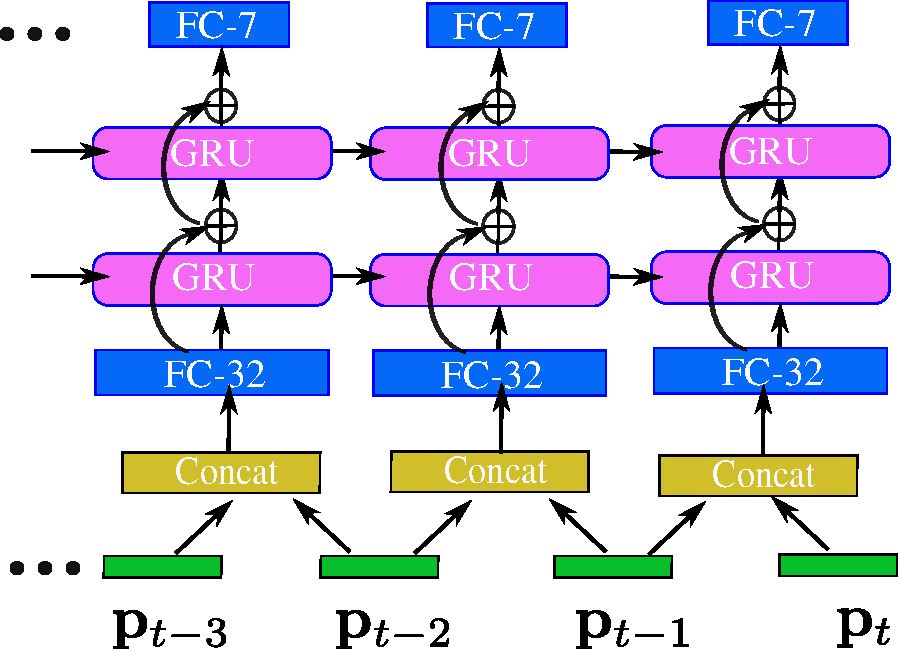
\includegraphics[width=\linewidth]{fig/RNN.pdf}
\end{center}
   \caption{The GRU RNN network architecture for modeling a sequence of camera poses.}
\label{fig:rnn}
\end{figure}

\textbf{Pose loss.}
Following the PoseNet~\cite{kendall2017geometric}, we use the geometric matching loss for training, which avoids the balancing factor between rotation and translation.
Formally, given a set of point cloud in 3D $~\hua{P}=\{\ve{x}\}$, and the loss for each image is written as,
\begin{align}
L(\ve{p}, \ve{p}^*) = \sum_{\ve{x} \in \hua{P}}\omega_{l_\ve{x}}|\pi(\ve{x}, \ve{p}) - \pi(\ve{x}, \ve{p}^*)|_2
\label{eq:proj_loss}
\end{align}
where $\ve{p}$ and $\ve{p}^*$ are the estimated pose and ground truth pose respectively. $\pi()$ is a projective function that maps a 3D point $\ve{x}$ to 2D image coordinates. $l_\ve{x}$ is the semantic label of $\ve{x}$ and $\omega_{l_\ve{x}}$ is a weight factor depended on the semantics. Here, we set stronger weights for point cloud belong to certain classes like traffic light, and we find it helps pose CNN to achieve better performance.
In~\cite{kendall2017geometric}, usually the 3D points that is visible by the camera are used by this loss to avoid very large numbers and ensure the stableness of training. However, online searching the visible 3D points from millions are unpractical.
Thus, we pre-render a depth map for each training image with a resolution of $256 \times 304$, based on its ground truth pose, and use the back projected 3D points from the depth map for training.

% Intuitively, we find the amount of points in each class is dramatically unbalanced, and most points are those on roads and trees. Nevertheless, the appearance variation of road and trees are not very sensitive to pose changes in the street-view scenario. In order to encourage the network to discover more str
% Thus,  other structures images like electricity pole or road light have rich structures like edges and textures, which potentially should be valued more for matching.
% In~\cite{ummenhofer2016demon}, the model try to predict a flow confidence map revealing the texture rich regions which helps pose estimation. In our work, we adopt the labelled semantic labels, and reweight each 3D point in the training loss, which drives the network to focus more on
% Thus, the learning loss changed to
% \begin{align}
% L(\ve{p}, \ve{p}^*) = \sum_{\ve{x} \in \hua{P}}\omega_{l_\ve{x}}|\pi(\ve{x}, \ve{p}) - \pi(\ve{x}, \ve{p}^*)|_2
% \label{eq:proj_loss}
% \end{align}
% where $\omega_{l_\ve{x}}$ is the weight of class $l_\ve{x}$. We set the weight for each class depends on the class edgeness which is the percentage of pixel along the edge
\subsection{Video parsing with pose guidance}
\label{subsec:parsing}
Having rectified pose at hand, one may direct render the semantic 3D world to the view of a camera, yielding a semantic parsing of the current image. However, the estimated pose is not perfect, alignment of very thin regions like light pole can totally miss sometimes. Other issues also exist such as many 3D points are missing due to reflection, \eg regions of building mirrors, and points can be sparse at long distance. Last, dynamic objects are not been able to be handled by the projected label map, yielding incorrect labelling. Thus, we propose an additional segment CNN to tackle these issues, while taking the rendered label map as segment priori as additional assistant.
% In our experiments, we show with pose rendered label map as an additional input, the segment results are temporally more consistent and yields better accuracy.

\begin{figure*}[]
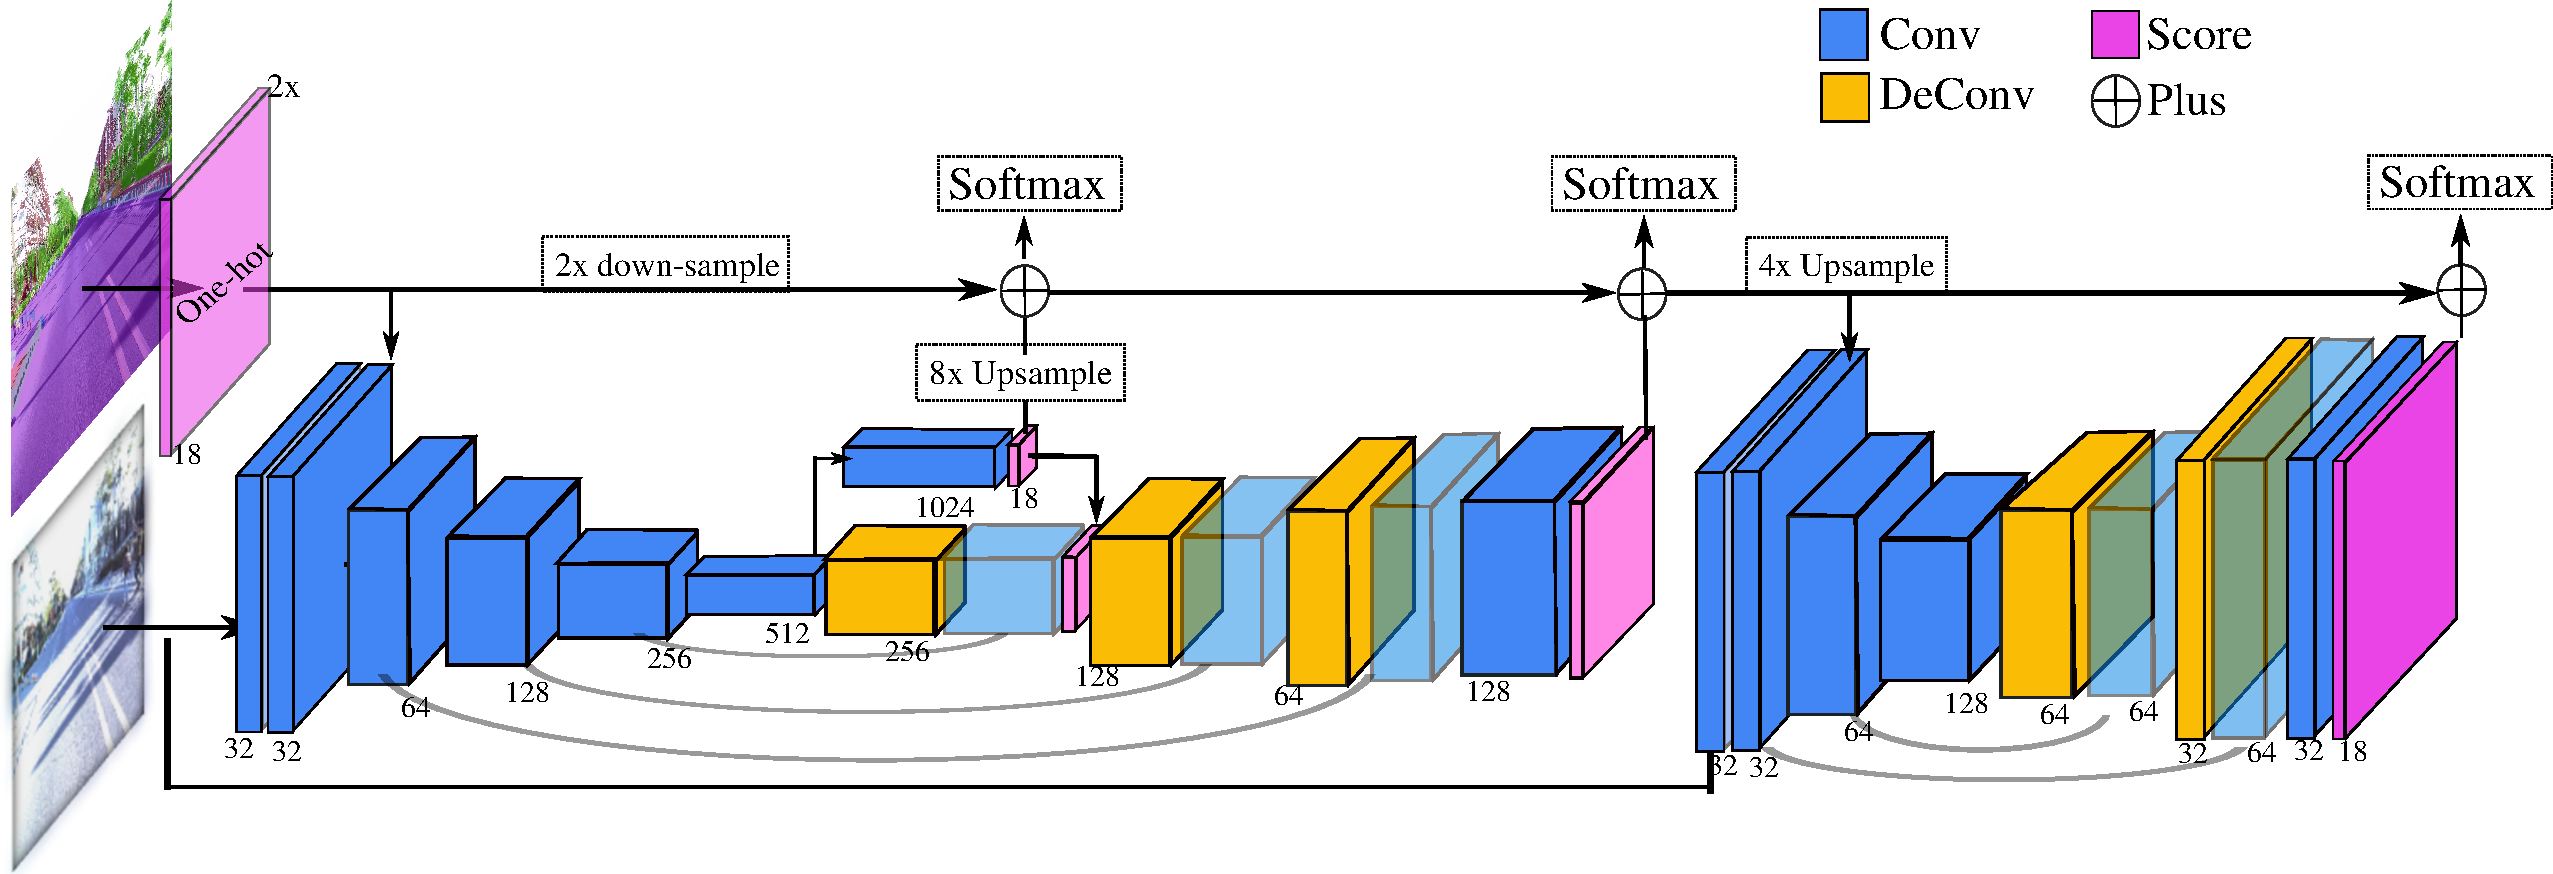
\includegraphics[width=\textwidth]{fig/segCNN.pdf}
\caption{Architecture of the segment CNN with rendered label map as a segmentation priori. At bottom of each convolutional block, we show the filter size, and at top we mark the downsample rates of each block \wrt the input image size. The 'softmax' text box indicates the places a loss is calculated. Details are in \secref{subsec:parsing}.}
\label{fig:segnet}
\end{figure*}

\paragraph{Segment network architecture.} As discussed in \secref{sec:related_work}, heavy parametrized networks like ResNet is not efficient enough for our online application. Thus, as illustrated in \figref{fig:segnet}, our segment CNN is a light weighted network containing an encoder-decoder network and a refinement network, and both have similar architecture with the corresponding ones used in DeMoN~\cite{ummenhofer2016demon}. However, due to that we have a segment prior from the 3D semantic map, we add a residual stream (top part of \figref{fig:segnet}), which encourages the network to learn the differences between the priori map with the ground truth. In~\cite{pohlen2016full}, a full resolution stream is used to keep spatial details, while at here, the rendered label map also helps to keep the semantic spatial layout.

Another notable difference for encoder-decoder network from DeMoN is that for network inputs, rather than directly concatenate the label map with input image, to balance the two, we first transform the label map to a score map through one-hot operation, and embed the score of each pixel to a 32 dimensional feature vector. Then, we concatenate this feature vector with the first layer output from image, and keeps the rest as the same with that in~\cite{ummenhofer2016demon}. For refinement network, we use the same strategy to handle the two inputs. Finally, the segment network produce a score map, yielding the semantic label of each pixel.

We train the segment network firstly with only RGB images, then fine-tune the network by adding the input of rendered label maps. This is because our network is trained from scratch, thus needs large amounts of data to learn effective features from images. However, the rendered label map from the estimated pose has on average 70$\%$ pixel accuracy, leaving only 30$\%$ of pixels having effective gradients. This could easily drive the network overfitting to the input label map, while slow down the process towards learning features from images. Finally, for segmentation loss, we use the standard softmax loss, and add intermediate supervision right after the outputs from both the encoder and the decoder as indicated in \figref{fig:segnet}. 